\documentclass{unswmaths}
\usepackage{unswshortcuts}
\usepackage{hyperref}
\begin{document}
\author{Adam J. Gray}
\title{Assignment 2}
\subject{Ergodic Theory}
\studentno{3329798}

\unswtitle

\section{}
\subsection{}
\begin{align*}
    T(\theta, \nu) = (\theta + \nu \mod 2\pi, \alpha\nu + \gamma \cos(\theta + \nu))
\end{align*}
\subsection{}
\begin{align*}
    J[T](\theta, \nu) = \left( 
    \begin{array}{cc}
        1   & 1 \\
        -\gamma \sin(\theta + \nu) & \alpha - \gamma\sin(\theta + \nu)
    \end{array}
    \right)
\end{align*}
and so
\begin{align*}
|J[T](\theta, \nu)| &= \alpha - \gamma\sin(\theta + \nu) + \gamma\sin(\theta + \nu) \\
    &= \alpha.
\end{align*}
So $ |J[T](\theta, \nu)| = 0 $ iff $ \alpha = 0 $. So since we have chosen $ \alpha > 0 $ this map is invertible everywhere by the inverse function theorem.
\subsection{}
\begin{figure}[h]
    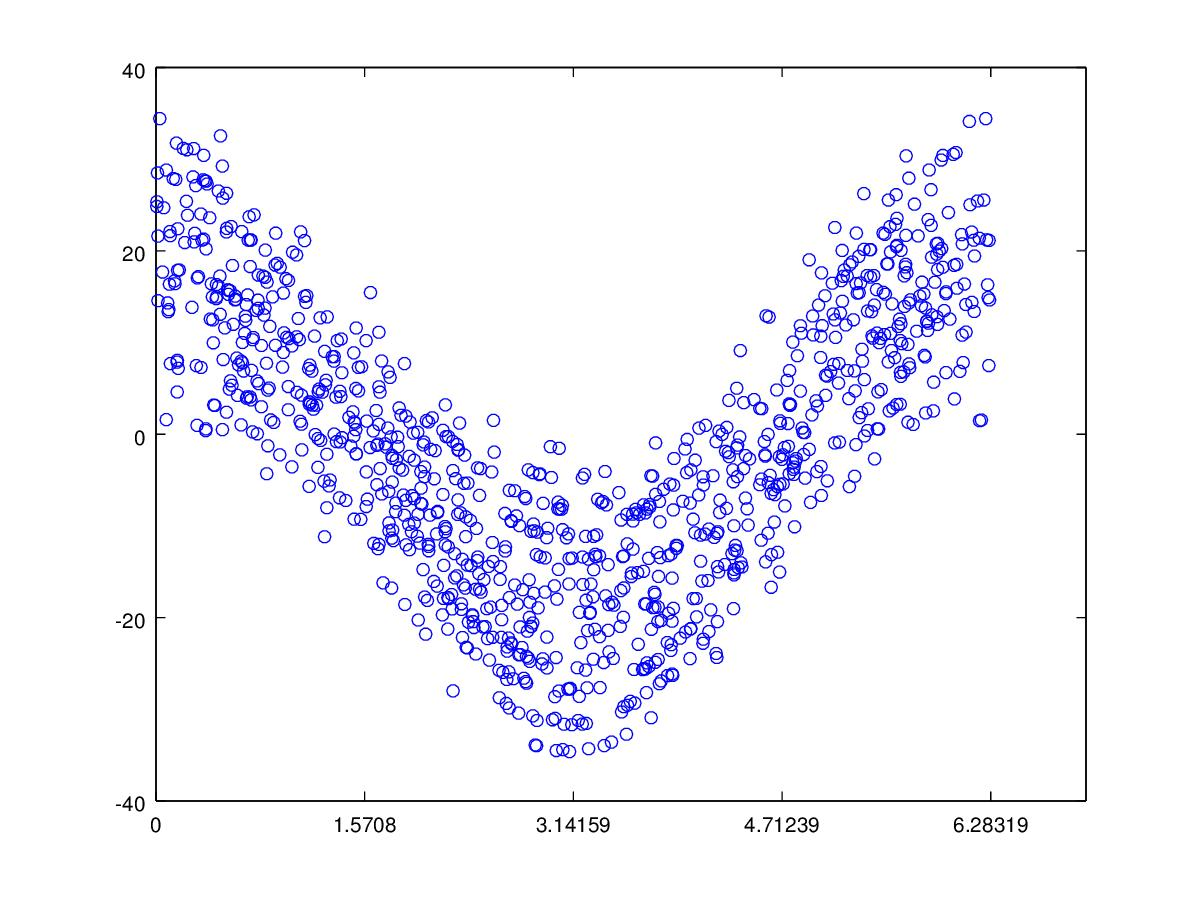
\includegraphics[scale=0.5]{Question_3}
    \caption{Phase plot of velocity vs table phase with $ \theta_0 = 0.5, \nu_0 = 0.5 $}
\end{figure}
\subsection{}
The maximum post-bounce velocities occur near $ \theta = 0 $ ($\theta = 2\pi$). This makes sense because the piston is traveling in the opposite direction to the ball. This is happening fastest at $ \theta = 0 $ and so this results in the largest bounces. The minimum is found at $ \theta = \pi $. This also makes sense because this is when the piston is traveling in the same direction as the ball. This is happening fastest at $ \theta = \pi $ and this results in the largest slowdown in the bounce.

\subsection{}
\subsection{}
\label{qn_6_ergodic}
\begin{figure}[h]
    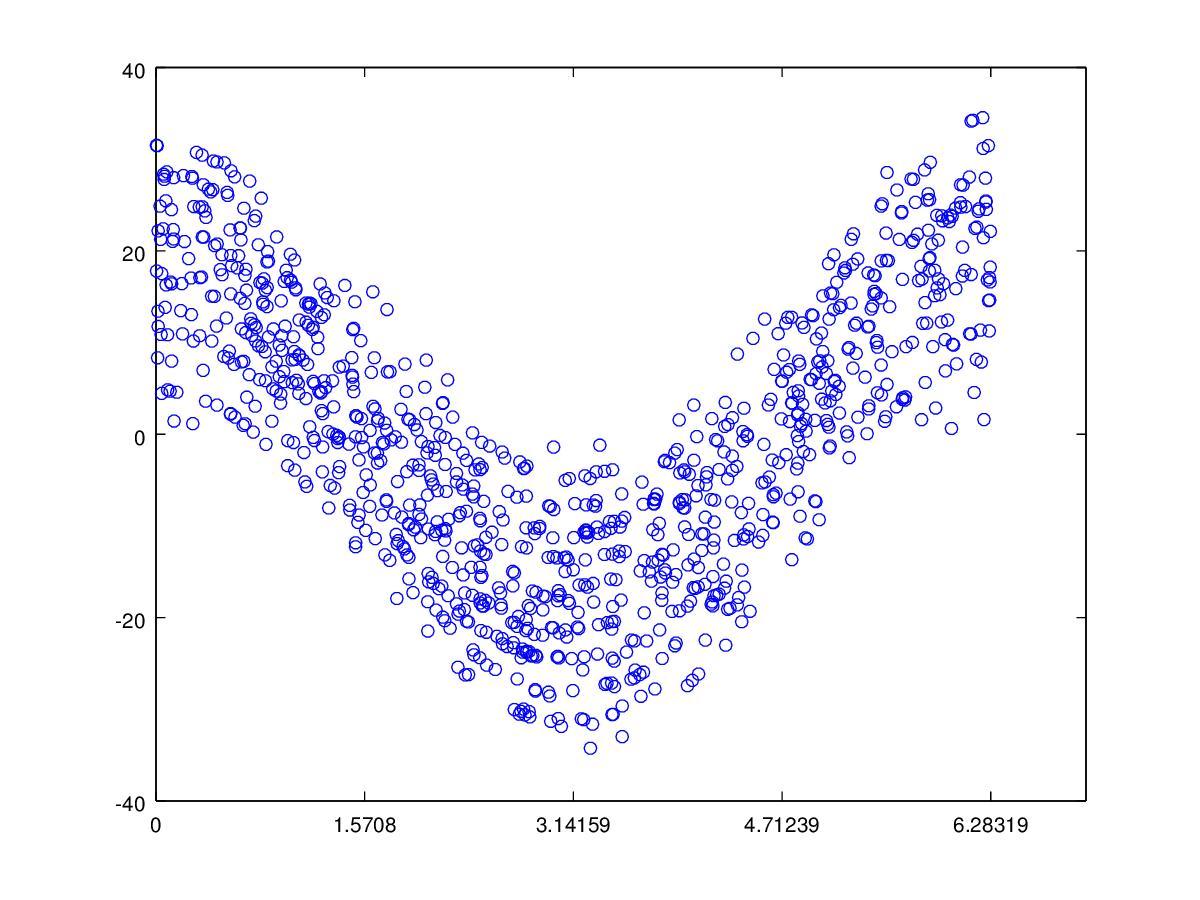
\includegraphics[scale=0.5]{Question_6_Ergodic}
    \caption{A bundle of 1000 points starting near $ \theta_0 = 0.5,  \nu_0 = 0.5 $ were iterated through $  T $ 10000 times}
\end{figure}

What figure 2 shows is that a small ball of points \emph{spreads out} in the phase space. Note that this ensemble of points roughly matches the orbit of one point. This would lead us to suspect that this process is Ergodic. 

\clearpage
\begin{figure}[h]
    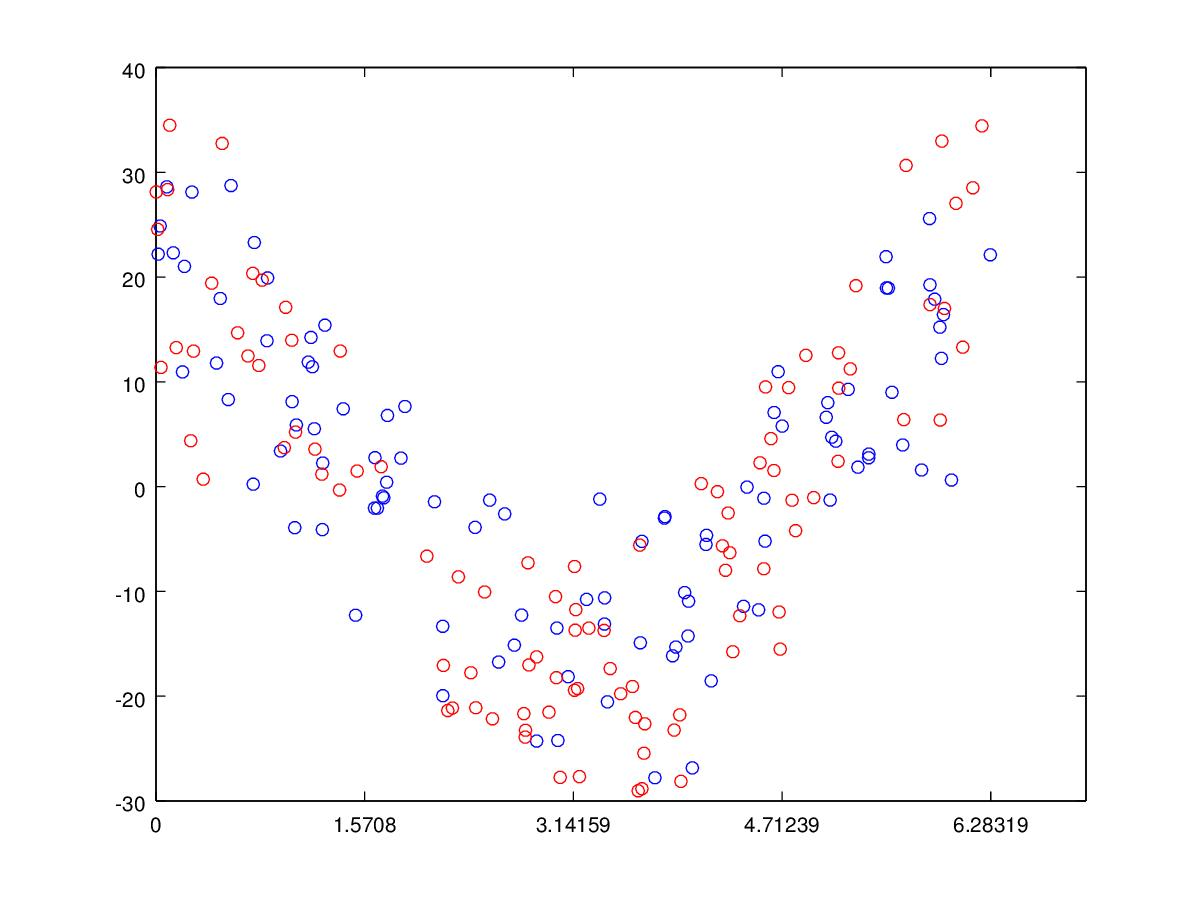
\includegraphics[scale=0.5]{Question_6_Mixing}
    \label{qn_6_mixing}
    \caption{Two bundles of 200 points after iterating through  $ T $ 10000 times. Blue started near $ \theta_0 = 0.5, \nu_0 = 0.5 $ while red started near $ \theta_0 = 1, \nu_0 = 1 $ }
\end{figure}


Figure 3 suggests that the long term behaviour of the  points is independent of their starting point. That is two sets of balls mix together. Although only testing with two bundles of balls is hardly rigerous, even empirically, this would suggest that this process is mixing.
\subsection{}
Since we suspect that this process is Ergodic (and mixing) this question can be answered by watching the long term behavior of 1 point. We do this for a point starting at $ \theta_0 = 0.5, \nu_0 = 0.5 $ and see that $ 49.95 \% $ of the first 10000 bounces occur when $ \theta < \pi / 2 $ or $ \theta > 3\pi / 2 $, that is when the piston is moving up. We conclude that there is equal chance of the ball hitting on a down stroke compared to an upstroke.

\subsection{}
Again since we suspect that this process is Ergodic we just study the evolution of one point.
We see that with $ \theta_0 = 0.5, \nu_0 = 0.5 $ the maximum $ \nu $ acheived is $ 34.821 $ and the 945 bounces are within $ 1\%$ of this velocity over $ 10^6 $ iterations. This suggests that ball is within $ 1\%$ of its maximum post bounce speed about $ 0.945\% $ of the time.

\section{}
\subsection{}
See code in \emph{PageRank.m} available at \url{https://github.com/adamjoshuagray/Honours_Ergodic_Theory/tree/master/Assignment_2/Project_2_Code}

\subsection{}
See code in \emph{Question\_2.m} avaiable at \url{https://github.com/adamjoshuagray/Honours_Ergodic_Theory/tree/master/Assignment_2/Project_2_Code}. 

The resultant vector is
\begin{align*}    q =
(  0.011878,
   0.016927,
   0.021698,
   0.021698,
   0.017105,
   0.025485,
   0.013031,
   0.017105, \\
   0.024870,
   0.027504,
   0.039333,
   0.013031,
   0.013898,
   0.025485,
   0.025485,
   0.021174, \\
   0.013031,
   0.013031,
   0.013031,
   0.015050,
   0.103970,
   0.011878,
   0.097454,
   0.111770,
   0.285079
)
\end{align*}
\subsection{}
See code in \emph{Question\_3.m} avaiable at \url{https://github.com/adamjoshuagray/Honours_Ergodic_Theory/tree/master/Assignment_2/Project_2_Code}. 

For $ p = 0.2 $ the resultant vector is
\begin{align*}
    q = (
   0.018891,
   0.020780,
   0.019820,
   0.019820,
   0.020144,
   0.020634,
   0.019139,
   0.020144, \\
   0.020823,
   0.021390,
   0.024838,
   0.019139,
   0.019647,
   0.020634,
   0.020634,
   0.021618, \\
   0.019139,
   0.019139,
   0.019139,
   0.019895,
   0.041789,
   0.018891,
   0.038559,
   0.041962,
   0.453391 
).
\end{align*}
For $ p = 0.5 $ the resultant vector is
\begin{align*}
    q = (
   0.015820,
   0.019775,
   0.019782,
   0.019782,
   0.018879,
   0.021813,
   0.016438,
   0.018879, \\
   0.021982,
   0.023395,
   0.030867,
   0.016438,
   0.017402,
   0.021813,
   0.021813,
   0.021951, \\
   0.016438,
   0.016438,
   0.016438,
   0.018020,
   0.071322,
   0.015820,
   0.065319,
   0.073702,
   0.379674 
).
\end{align*}
\begin{figure}[h]
    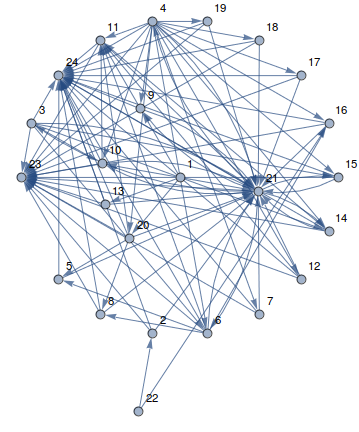
\includegraphics[scale=0.8]{Graph}
    \caption{The layout of the network}
\end{figure}
In figure 4 we see that there are basically 3 important nodes, 21, 23 and 24. When choosing a smaller value for $ p $ less weight is given to 21 and 23 and all of it goes to 24. As we might want to keep 21 and 23 as important nodes we would select a higher value of $ p $. Say $ p = 0.85 $.
To see a comparison of different weightings given for different values of $ p $ see figure 5.

\begin{figure}[h]
    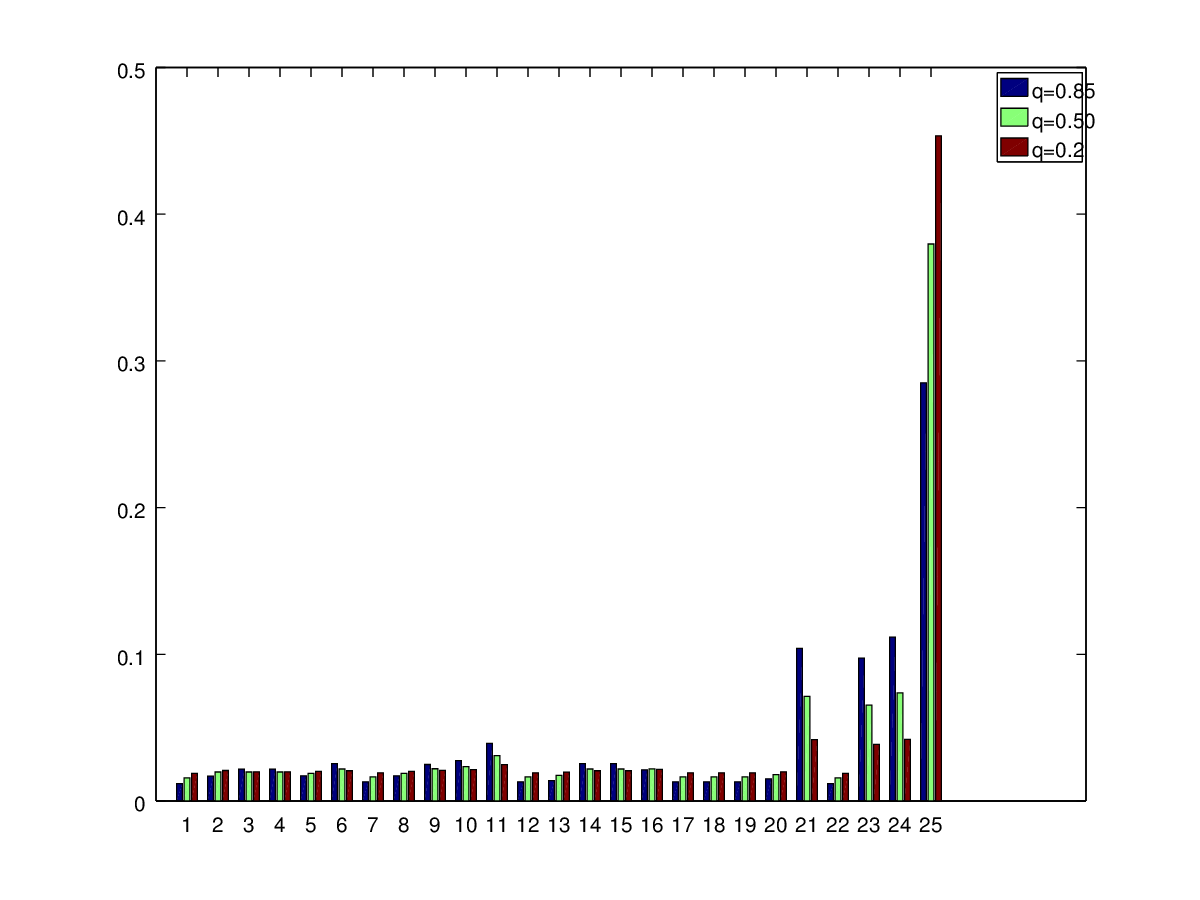
\includegraphics[scale=0.7]{Different_ps}
    \caption{Different weightings for different values of $ p $.}
\end{figure}
\clearpage
\subsection{}
See code in \emph{Question\_4.m} avaiable at \url{https://github.com/adamjoshuagray/Honours_Ergodic_Theory/tree/master/Assignment_2/Project_2_Code}. 

The solution converges exponentially with the error at step n given by
\begin{align*}
    Error(n) = \exp(-0.48640n - 0.25550).
\end{align*}
This is true for about $ n \leq 65 $, after that the error has reached machine precision and cannot improve any further.
See figure 6 for a plot of $ \log(Error(n)) $.

\begin{figure}[h]
    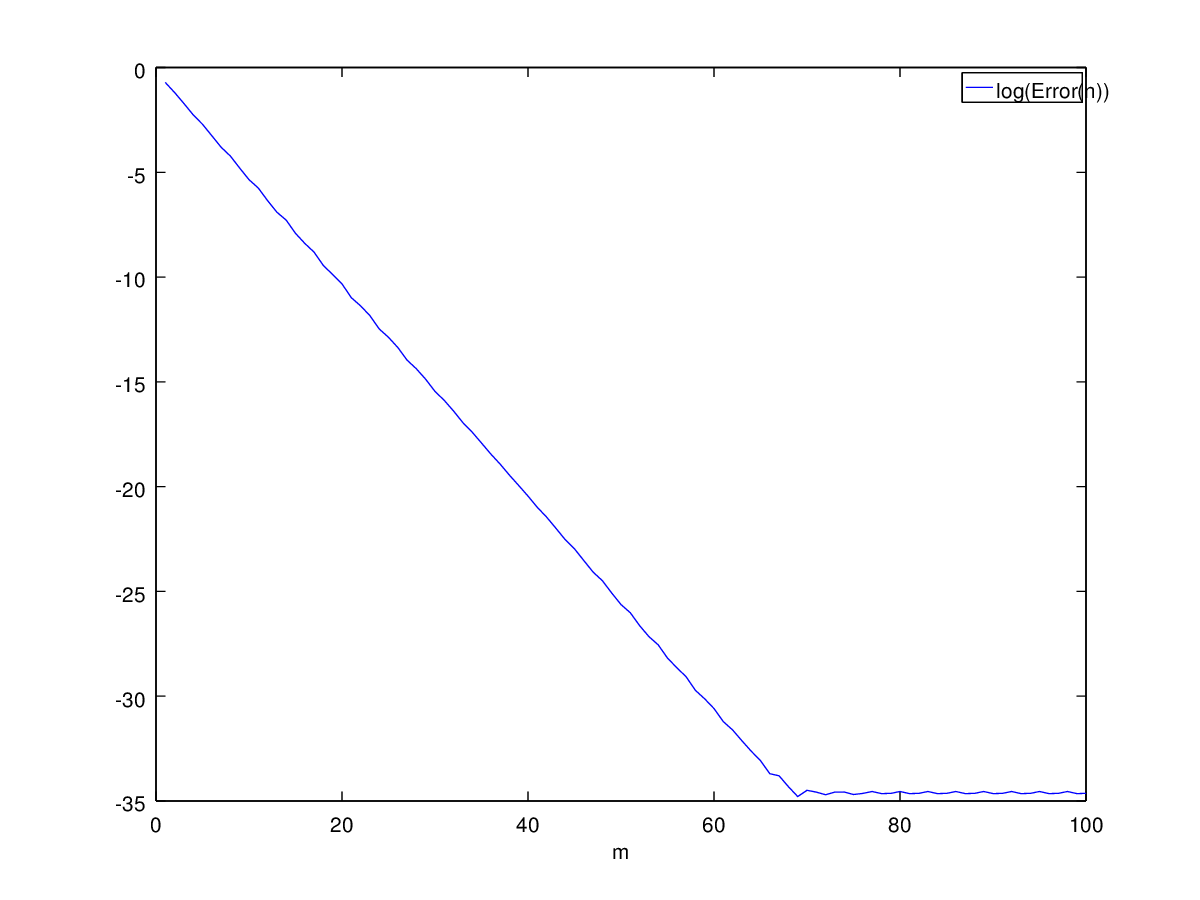
\includegraphics[scale=0.5]{Log_Error_n}
    \caption{Exponential convergence to the stationary vector. Note that at about $n = 65 $ the graph flattens out. This is because the error has reached machine precision.}
\end{figure}

\subsection{}
\subsubsection{}
See code in \emph{PageRank2.m} avaiable at \url{https://github.com/adamjoshuagray/Honours_Ergodic_Theory/tree/master/Assignment_2/Project_2_Code}. 
\subsubsection{}
See code in \emph{Question\_5\_b.m} avaiable at \url{https://github.com/adamjoshuagray/Honours_Ergodic_Theory/tree/master/Assignment_2/Project_2_Code}. 

\begin{align*}
    q = (
   0.023011,
   0.029826,
   0.031190,
   0.031190,
   0.028626,
   0.034984,
   0.024166,
   0.028626, \\
   0.035070,
   0.037710,
   0.051047,
   0.024166,
   0.025737,
   0.034984,
   0.034984,
   0.033940, \\
   0.024166,
   0.024166,
   0.024166,
   0.026891,
   0.124281,
   0.023011,
   0.114333,
   0.129734
)
\end{align*}
\begin{figure}[h]
    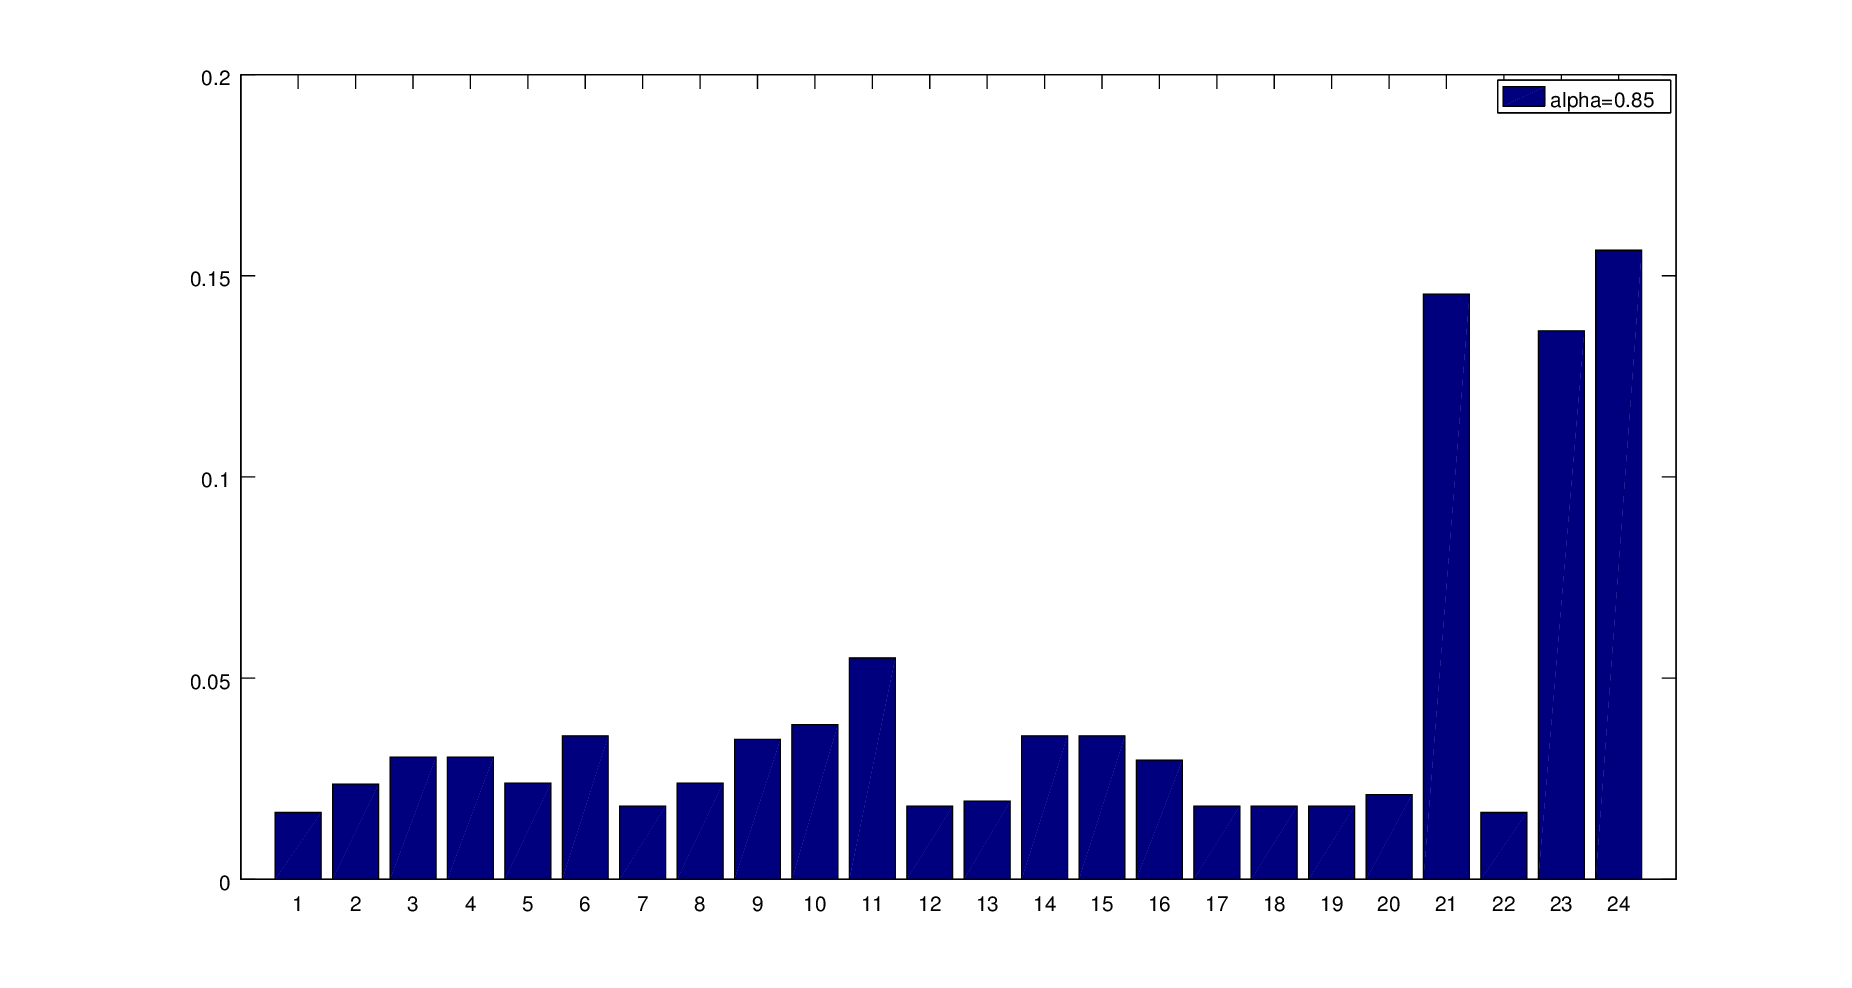
\includegraphics[scale=0.4]{Second_Rank}
    \caption{The page rank weightings for this network using the second page rank algorithm.}
\end{figure}


We can see from figure 7 and by comparing to figure 5, that the this second page rank method results in a more \emph{uniform} distribution or page ranks. This is because there is a \emph{lattent} connectivity between all pages introduced by the probability of just going to a random page, regardless of the links. This means that each page is \emph{one hop} away from every other page, instead of two hops in the case of the first method. As each page is more connected we would expect a more uniform page rank distribution as we have observed here.
\subsubsection{}
See code in \emph{Question\_5\_c.m} avaiable at \url{https://github.com/adamjoshuagray/Honours_Ergodic_Theory/tree/master/Assignment_2/Project_2_Code}. 

The solution converges exponentially with the error at step $ n $ given by
\begin{align*}
    Error(n) = \exp(-1.04629n - 0.25217).
\end{align*}
This is true for about $ n \leq 30 $, after that the error has reached machine precisiion and cannot improce any further. See figure 8 for a plot of $ \log(Errror(n)) $.

\begin{figure}[h]
    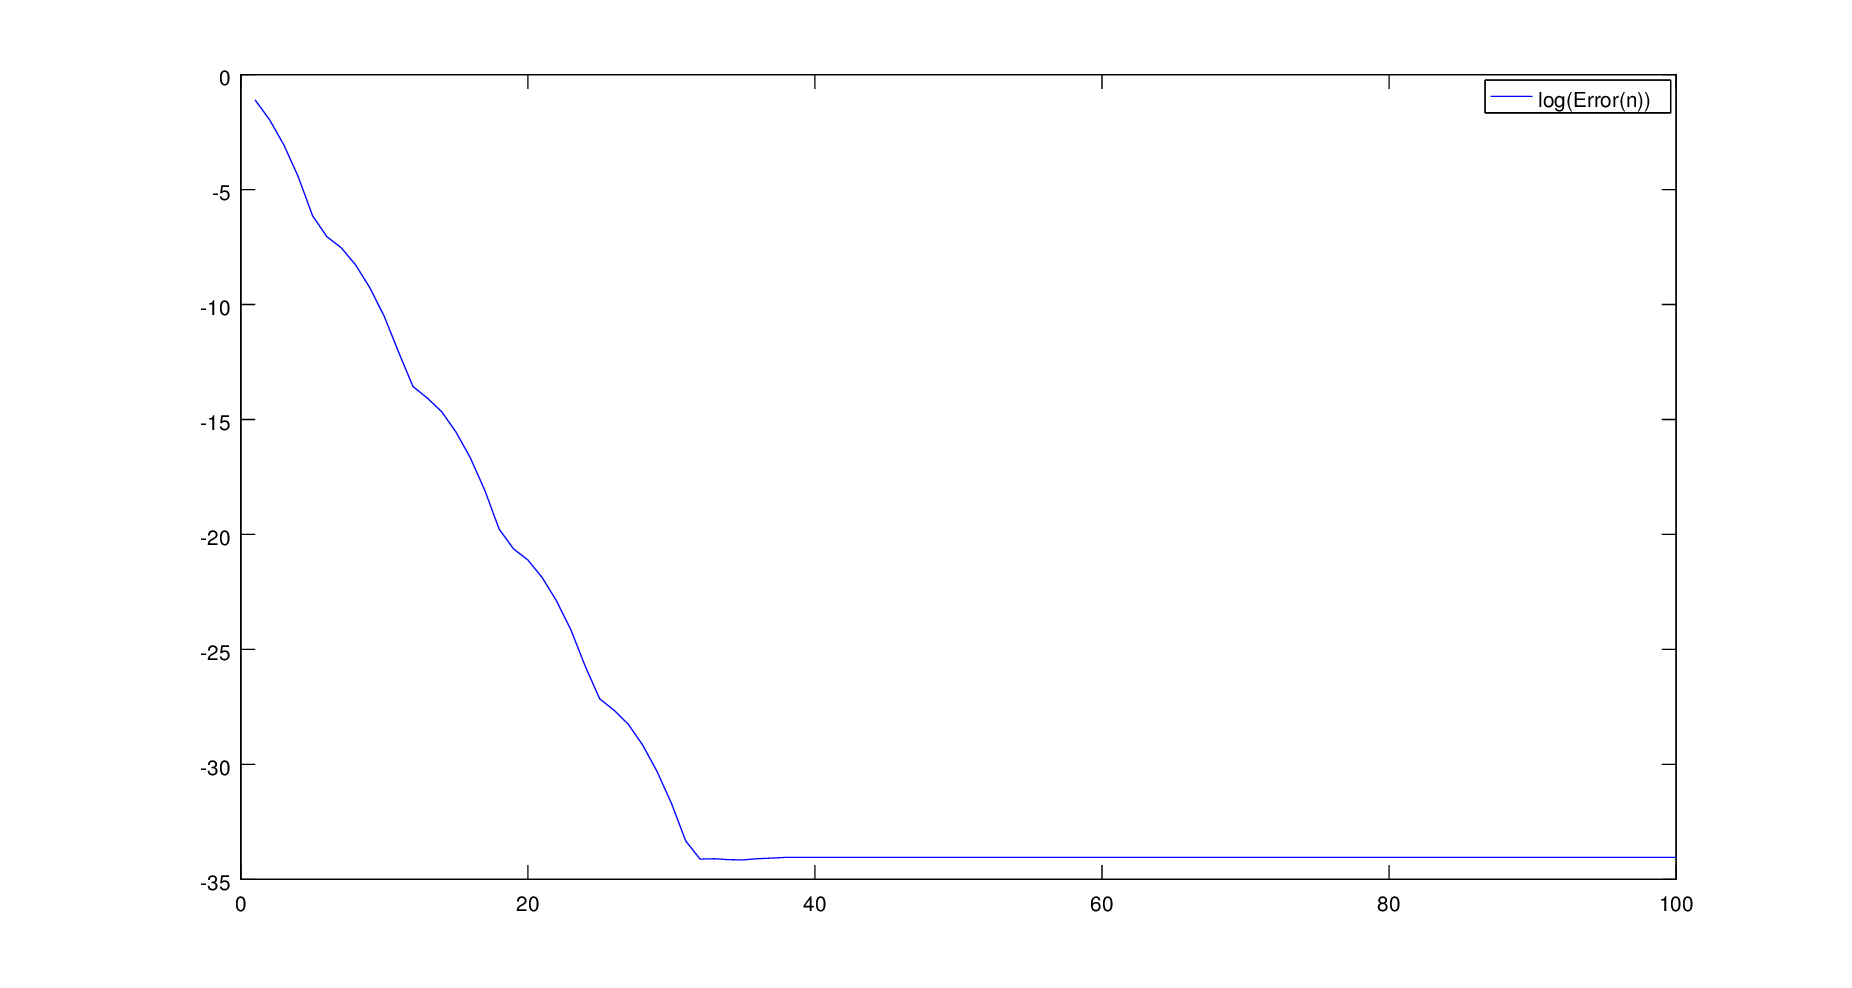
\includegraphics[scale=0.5]{Log_Error_n_2}
    \caption{Exponential convergence to the stationary vector. Note that at about $n = 30 $ the graph flattens out. This is because the error has reached machine precision.}
\end{figure}
It converges faster because the uniform distribution is in a \emph{1 norm} sense, \emph{closer} to $ q $ than in the first case. It also converges a bit faster because the matrix $ G $ is slightly smaller than the matrix $ Q $.
\end{document}
